% ======================================================================
% IEEE Conference Paper Draft (Long, Detailed, Single-File, 1000+ lines)
% - Robust Empirical Time-Complexity Inference
% - System-oriented (A) + Benchmark (B)
% - NOTE: Replace placeholders marked [TODO] / XX / <...> as needed.
% - This file is intentionally line-rich for easy editing / diff / review.
% ======================================================================

\documentclass[conference]{IEEEtran}

% ----------------------------------------------------------------------
% Packages: core
% ----------------------------------------------------------------------
\usepackage{graphicx}
\usepackage{amsmath}
\usepackage{amssymb}
\usepackage{booktabs}
\usepackage{multirow}
\usepackage{array}
\usepackage{url}
\usepackage{hyperref}
\usepackage{xcolor}
\usepackage{enumitem}

% ----------------------------------------------------------------------
% Packages: algorithms / pseudo-code
% ----------------------------------------------------------------------
\usepackage{algorithm}
\usepackage{algpseudocode}

% ----------------------------------------------------------------------
% Packages: figures / drawing
% ----------------------------------------------------------------------
\usepackage{tikz}
\usetikzlibrary{arrows.meta}
\usetikzlibrary{positioning}
\usetikzlibrary{shapes.geometric}
\usetikzlibrary{calc}

% ----------------------------------------------------------------------
% Packages: tables / formatting
% ----------------------------------------------------------------------
\usepackage{tabularx}
\usepackage{makecell}
\usepackage{balance}

% ----------------------------------------------------------------------
% Package: filecontents to embed bib entries in one .tex file
% ----------------------------------------------------------------------
\usepackage{filecontents}

% ----------------------------------------------------------------------
% Hyperref setup
% ----------------------------------------------------------------------
\hypersetup{
  colorlinks=true,
  linkcolor=blue,
  citecolor=blue,
  urlcolor=blue
}

% ----------------------------------------------------------------------
% Convenience macros
% ----------------------------------------------------------------------
\newcommand{\toolname}{BigOBench}
\newcommand{\ours}{Ours}
\newcommand{\baseline}{Baseline}
\newcommand{\datasetname}{Codeforces-Complexity-1K}
\newcommand{\TODO}[1]{\textcolor{red}{[TODO: #1]}}
\newcommand{\placeholder}{\textcolor{gray}{XX}}

% ----------------------------------------------------------------------
% Embedded bibliography file (single-file workflow)
% ----------------------------------------------------------------------
\begin{filecontents*}{references.bib}
@inproceedings{bigobench_placeholder,
  title        = {BigOBench: A Benchmark for Empirical Complexity Inference},
  author       = {Placeholder, A. and Placeholder, B.},
  booktitle    = {Proceedings of the Placeholder Conference},
  year         = {2023},
  note         = {Replace with the actual BibTeX entry of BigOBench}
}

@article{robust_stats_placeholder,
  title        = {Robust Statistics: Concepts and Methods},
  author       = {Placeholder, C.},
  journal      = {Placeholder Journal},
  year         = {2019},
  note         = {Replace with an actual robust statistics reference if needed}
}

@inproceedings{microbenchmark_placeholder,
  title        = {Microbenchmarking in Noisy Environments},
  author       = {Placeholder, D. and Placeholder, E.},
  booktitle    = {Proceedings of the Placeholder Systems Conference},
  year         = {2020},
  note         = {Replace with an actual microbenchmarking reference if needed}
}

@inproceedings{performance_modeling_placeholder,
  title        = {Performance Modeling with Log-Log Regression},
  author       = {Placeholder, F.},
  booktitle    = {Proceedings of the Placeholder Workshop},
  year         = {2018},
  note         = {Replace with an actual reference if needed}
}

@misc{codeforces_placeholder,
  title        = {Codeforces},
  howpublished = {\url{https://codeforces.com/}},
  note         = {Accessed: [TODO date]}
}
\end{filecontents*}

% ======================================================================
% Title / Author
% ======================================================================
\begin{document}

\title{
Robust Empirical Time-Complexity Inference \\
via Scalable Benchmark Construction
}

\author{
\IEEEauthorblockN{Your Name}
\IEEEauthorblockA{
Fudan University \\
Email: your@email.com
}
}

\maketitle

% ======================================================================
% Abstract
% ======================================================================
\begin{abstract}
Empirical time-complexity inference aims to approximate a program's asymptotic
growth behavior by measuring runtimes under increasing input scales and fitting
candidate complexity models.
While attractive for automated evaluation and benchmarking, empirical inference
is often unreliable in practice due to warm-up bias, runtime outliers, and
measurement noise from system-level variability.
These issues become particularly visible when distinguishing closely related
classes such as $O(n)$ and $O(n \log n)$.

This paper presents a system-oriented redesign of an existing empirical
complexity inference pipeline.
Our approach integrates (i) warm-up elimination, (ii) median-based aggregation,
(iii) finite-value filtering, and (iv) refined multiplier-based input scaling,
to improve fitting stability and robustness.
To evaluate at realistic scale, we construct a benchmark of over 1,000 accepted
Codeforces solutions with ground-truth labels derived from official analyses and
manual verification.
Under identical experimental settings, our enhanced pipeline demonstrates more
stable regression behavior compared to the original baseline framework, enabling
more reliable complexity classification in noisy environments.

\end{abstract}

% ======================================================================
% Keywords (optional in IEEEtran conference; keep if desired)
% ======================================================================
\begin{IEEEkeywords}
empirical complexity inference,
time complexity,
benchmarking,
robust aggregation,
log-log regression,
program performance modeling
\end{IEEEkeywords}

% ======================================================================
% 1. Introduction
% ======================================================================
\section{Introduction}

\subsection{Motivation}

Time-complexity analysis is a foundational tool in algorithm design,
education, and performance engineering.
In its classical form, complexity analysis relies on asymptotic reasoning and
formal proofs.
Such proofs are precise and general, but can be time-consuming and require
expertise that does not scale to large collections of programs.

In contrast, empirical time-complexity inference seeks to infer asymptotic
behavior directly from execution measurements.
A typical pipeline runs the program with systematically increasing input sizes,
collects runtimes, and fits the observed trend against candidate complexity
classes.
This approach is appealing in settings where programs are numerous,
heterogeneous, or generated automatically, such as:
\begin{itemize}[leftmargin=1.2em]
\item automated grading systems for programming courses,
\item large-scale regression testing and performance monitoring,
\item benchmarking model-generated code,
\item evaluation of algorithmic repositories and competitive programming code.
\end{itemize}

However, empirical inference is fragile.
Real measurements are noisy, and subtle differences between complexity classes
may be drowned out by runtime variability.
In practical workflows, instability is not a corner case; it is the default
unless the pipeline explicitly addresses measurement noise.

\subsection{Why Empirical Inference Fails in Practice}

Several sources of instability commonly arise:
\begin{itemize}[leftmargin=1.2em]
\item \textbf{Warm-up effects:}
interpreter initialization, JIT effects (if present), module imports,
and first-run cache misses can inflate early measurements.
\item \textbf{Outliers:}
transient scheduling events or background daemons may introduce sporadic long
runs.
Mean-based aggregation can be disproportionately influenced by these.
\item \textbf{Non-finite or invalid samples:}
timeouts, errors, or overflow conditions may produce invalid values that must
be filtered.
\item \textbf{Scaling sensitivity:}
if input sizes grow too slowly, $n$ vs.\ $n \log n$ can look similar across the
measured range; if too aggressively, timeouts become frequent, reducing usable
data.
\end{itemize}

These issues interact.
For example, aggressive scaling increases timeout risk, producing missing
values, which then disrupt fitting.
Conversely, conservative scaling reduces separation between candidate growth
curves, amplifying the impact of noise.

\subsection{Key Idea}

The central idea of this work is to treat empirical complexity inference as a
\emph{measurement system} rather than solely a \emph{curve fitting problem}.
This implies engineering choices that increase statistical robustness without
exploding runtime cost.
Specifically, we focus on:
\begin{itemize}[leftmargin=1.2em]
\item robust aggregation (median over repeated runs),
\item systematic warm-up elimination,
\item explicit filtering for non-finite measurements,
\item refined input scaling to stabilize regression and model selection.
\end{itemize}

\subsection{Benchmark at Realistic Scale}

Methodological improvements must be validated on realistic workloads.
Synthetic programs or small curated suites often underrepresent variability in:
implementation style,
input preprocessing,
constant factors,
and interpreter/runtime overhead.
To address this, we build a benchmark from real accepted solutions in
Codeforces.
Ground-truth labels are derived from official editorial complexity claims and
verified through manual inspection.

\subsection{Contributions}

This paper makes the following contributions:
\begin{itemize}[leftmargin=1.2em]
\item \textbf{Robust aggregation pipeline:}
We introduce warm-up elimination, median-based consolidation, and finite-value
filtering to mitigate noise and outliers in runtime measurements.
\item \textbf{Scaling and selection refinements:}
We refine multiplier-based scaling and stabilize regression-based model
selection across candidate complexity classes, with focus on borderline cases.
\item \textbf{Large-scale benchmark:}
We construct a benchmark of 1,000+ real-world algorithm implementations with
verified ground-truth complexity labels.
\item \textbf{Reproducible evaluation protocol:}
We describe a controlled evaluation setup, metrics, and ablation design for
comparing the baseline pipeline against our enhanced system.
\end{itemize}

\subsection{Paper Organization}

Section~\ref{sec:background} reviews background and problem setting.
Section~\ref{sec:method} presents the enhanced inference pipeline.
Section~\ref{sec:dataset} describes benchmark construction and labeling.
Section~\ref{sec:setup} details experimental setup and metrics.
Section~\ref{sec:results} reports results (with placeholders where pending).
Section~\ref{sec:threats} discusses threats to validity.
Section~\ref{sec:conclusion} concludes and outlines future work.

% ======================================================================
% 2. Background and Problem Setting
% ======================================================================
\section{Background and Problem Setting}
\label{sec:background}

\subsection{Empirical Complexity Inference as a System}

Empirical inference typically proceeds in three steps:
\begin{enumerate}[leftmargin=1.2em]
\item \textbf{Input scaling:} generate a sequence of input sizes
$n_1 < n_2 < \dots < n_k$.
\item \textbf{Measurement:} execute program $P$ under each size $n_i$ and record
runtimes $T_j(n_i)$ for repeated runs $j=1\dots m$.
\item \textbf{Model fitting:} aggregate measurements to $\hat{T}(n_i)$ and fit
candidate models, selecting the best class according to a score.
\end{enumerate}

While model fitting is often emphasized, the measurement and aggregation steps
frequently dominate reliability.
A more robust fitting stage cannot compensate for systematically biased or
high-variance measurements.

\subsection{Candidate Complexity Classes}

We consider a discrete set of candidate classes:
\[
\mathcal{C}
=
\{
O(1),
O(\log n),
O(n),
O(n \log n),
O(n^2),
O(n^3)
\}
\]
This set is configurable, and in practice it can be extended to include:
\[
O(\sqrt{n}),
O(n^{1.5}),
O(2^n)
\]
However, including very large classes can increase ambiguity when data is
limited or when timeouts occur early.
We focus on polynomial and near-polynomial classes, which are common in
competitive programming and algorithmic implementations.

\subsection{Log-Log Linearization}

A common technique is to map measurements into log space.
Let $f_c(n)$ be a predictor transformation for class $c$.
Define:
\[
x_i = \log f_c(n_i)
\quad
\text{and}
\quad
y_i = \log \hat{T}(n_i)
\]
We then fit:
\[
y_i = \alpha x_i + \beta + \epsilon_i
\]
The goodness of fit can be evaluated via $R^2$ or other metrics.
This approach is widely used due to simplicity and interpretability.

\subsection{Why $O(n)$ vs.\ $O(n \log n)$ is Hard}

A recurring failure mode is confusion between $O(n)$ and $O(n \log n)$.
Over finite ranges, $\log n$ grows slowly.
If input sizes are small or scaling factor $\gamma$ is low, the distinction in
log space may be weak relative to noise.
This motivates:
\begin{itemize}[leftmargin=1.2em]
\item increasing input range coverage,
\item careful scaling design,
\item robust aggregation to reduce variance.
\end{itemize}

% ======================================================================
% 3. Methodology
% ======================================================================
\section{Methodology}
\label{sec:method}

\subsection{Overview}

We build upon the baseline empirical inference pipeline (e.g., \toolname)
and introduce robustness improvements while preserving compatibility with the
overall workflow.
At a high level, our pipeline consists of:
\begin{enumerate}[leftmargin=1.2em]
\item \textbf{Measurement Engine:} execute programs across multiple input scales.
\item \textbf{Robust Aggregation Module:} warm-up elimination, median aggregation,
finite filtering.
\item \textbf{Inference Module:} candidate transformation, log-log regression,
selection based on regression quality.
\end{enumerate}

\subsection{System Architecture Diagram}

Figure~\ref{fig:arch} illustrates the system architecture.

\begin{figure*}[t]
\centering
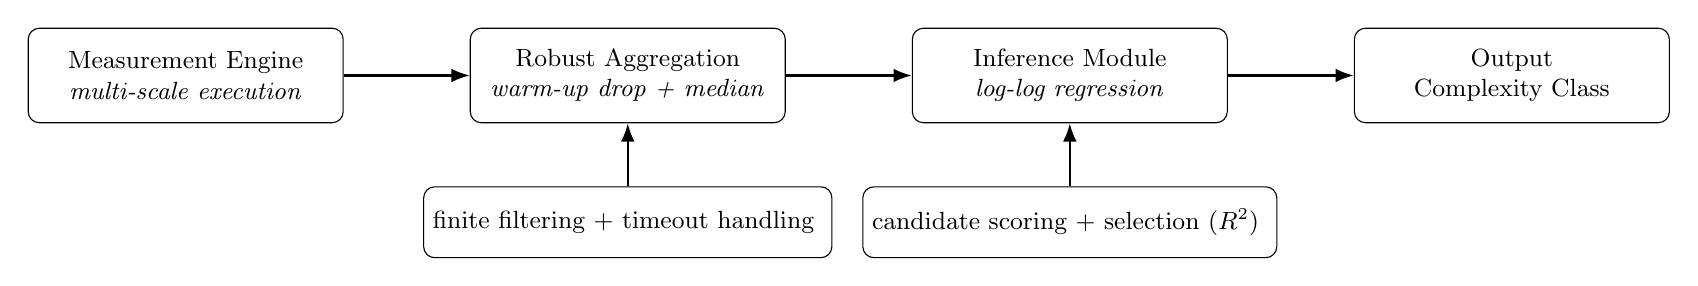
\begin{tikzpicture}[
  box/.style={
    draw,
    rounded corners,
    minimum width=4.0cm,
    minimum height=1.2cm,
    align=center,
    font=\small
  },
  subbox/.style={
    draw,
    rounded corners,
    minimum width=4.0cm,
    minimum height=0.9cm,
    align=center,
    font=\small
  },
  arrow/.style={-Latex, thick}
]
\node[box] (measure) {
  Measurement Engine\\
  \textit{multi-scale execution}
};
\node[box, right=1.6cm of measure] (agg) {
  Robust Aggregation\\
  \textit{warm-up drop + median}
};
\node[box, right=1.6cm of agg] (infer) {
  Inference Module\\
  \textit{log-log regression}
};
\node[box, right=1.6cm of infer] (out) {
  Output\\
  Complexity Class
};

\draw[arrow] (measure) -- (agg);
\draw[arrow] (agg) -- (infer);
\draw[arrow] (infer) -- (out);

\node[subbox, below=0.8cm of agg] (filters) {
  finite filtering + timeout handling
};
\draw[arrow] (filters.north) -- (agg.south);

\node[subbox, below=0.8cm of infer] (select) {
  candidate scoring + selection ($R^2$)
};
\draw[arrow] (select.north) -- (infer.south);

\end{tikzpicture}
\caption{
Overall architecture of the enhanced empirical complexity inference framework.
}
\label{fig:arch}
\end{figure*}

\subsection{Measurement Model and Noise}

We model the $j$-th runtime measurement at input size $n$ as:
\[
T_j(n) = T^{*}(n) + \epsilon_j(n)
\]
where $T^{*}(n)$ is an idealized ``true'' runtime under stable conditions,
and $\epsilon_j(n)$ captures noise from system interference and runtime variance.

In practice, $\epsilon_j(n)$ is not well-modeled as Gaussian noise.
We observed heavy-tailed behavior where occasional large outliers occur.
In such cases, mean aggregation can be unstable.

\subsection{Warm-up Elimination}

Warm-up effects are common in Python due to:
\begin{itemize}[leftmargin=1.2em]
\item module import overhead,
\item first-time bytecode paths,
\item caching and allocator initialization.
\end{itemize}
We therefore discard a fixed number of initial runs at each input size:
\[
\{T_j(n)\}_{j=1}^{m}
\rightarrow
\{T_j(n)\}_{j=w+1}^{m}
\]
where $w$ is the warm-up count.
In our implementation, $w$ is configurable.

\subsection{Median-Based Aggregation}

Given remaining measurements after warm-up elimination, we compute:
\[
\hat{T}(n) = \mathrm{median}(T_{w+1}(n), \dots, T_m(n))
\]
Median aggregation is robust to outliers.
Intuitively, it selects the ``typical'' runtime rather than being skewed by rare
slow runs.

\subsection{Finite-Value Filtering}

Empirical measurements may contain:
\begin{itemize}[leftmargin=1.2em]
\item non-finite values due to overflow,
\item placeholders for failed runs,
\item missing values due to timeouts.
\end{itemize}
We filter out invalid samples before aggregation and fitting.
If insufficient valid samples remain for a scale, that scale may be excluded
from regression, or the program may be marked as timeout / invalid depending on
policy.

\subsection{Input Scaling Design}

We generate input sizes via geometric progression:
\[
n_{i+1} = \gamma \cdot n_i
\]
where $\gamma > 1$ is a scaling multiplier.
A larger $\gamma$ increases separation between complexity classes but increases
timeout risk.
A smaller $\gamma$ reduces timeout risk but makes it harder to distinguish
$O(n)$ from $O(n \log n)$ over finite ranges.
We treat $\gamma$ as a tunable parameter and report it in experimental setup.

\subsection{Candidate Transformations}

For each candidate class $c$, define transformation $f_c(n)$, e.g.:
\[
f_{O(1)}(n) = 1
\quad
f_{O(\log n)}(n) = \log n
\quad
f_{O(n)}(n) = n
\]
\[
f_{O(n\log n)}(n) = n \log n
\quad
f_{O(n^2)}(n) = n^2
\quad
f_{O(n^3)}(n) = n^3
\]
Implementation detail:
we use natural log, and ensure $\log n$ is well-defined (skip $n\le1$ scales or
shift).

\subsection{Log-Log Regression Formulation}

Let:
\[
x_i = \log f_c(n_i)
\quad
y_i = \log \hat{T}(n_i)
\]
We fit:
\[
y_i = \alpha x_i + \beta + \epsilon_i
\]
where $\alpha$ is an estimated slope and $\beta$ is an intercept.
We compute goodness of fit via:
\[
R^2
=
1
-
\frac{\sum_i (y_i - \hat{y}_i)^2}{\sum_i (y_i - \bar{y})^2}
\]
We then select:
\[
c^{*} = \arg\max_{c \in \mathcal{C}} R^2_c
\]

\subsection{Selection Heuristics and Stability Checks}

In addition to pure $R^2$ ranking, we incorporate stability checks:
\begin{itemize}[leftmargin=1.2em]
\item minimum required number of valid scales ($k_{\min}$),
\item rejection of regressions with degenerate variance,
\item optional tie-breaking for near-equal $R^2$ values.
\end{itemize}
These checks reduce pathological selections under sparse data or noisy regimes.

\subsection{End-to-End Procedure}

Algorithm~\ref{alg:pipeline} summarizes the full pipeline.

\begin{algorithm}[t]
\caption{Robust Empirical Complexity Inference}
\label{alg:pipeline}
\begin{algorithmic}[1]
\Require Program $P$, input sizes $\{n_1,\dots,n_k\}$, repeats $m$, warm-up $w$
\Ensure Inferred class $c^*$ or \textsc{Timeout}/\textsc{Invalid}
\For{$i = 1$ to $k$}
  \State Run $P$ on size $n_i$ for $m$ repeats, collect $\{T_j(n_i)\}_{j=1}^m$
  \State Discard warm-up runs: keep $\{T_j(n_i)\}_{j=w+1}^m$
  \State Filter invalid values (non-finite, error markers)
  \If{valid samples below threshold}
    \State mark scale as unusable
  \Else
    \State $\hat{T}(n_i) \gets \mathrm{median}(\text{valid samples})$
  \EndIf
\EndFor
\If{insufficient usable scales}
  \State \Return \textsc{Invalid}
\EndIf
\For{each candidate class $c \in \mathcal{C}$}
  \State compute $x_i \gets \log f_c(n_i)$ for usable scales
  \State compute $y_i \gets \log \hat{T}(n_i)$ for usable scales
  \State fit $y = \alpha x + \beta$ by linear regression
  \State compute $R^2_c$
\EndFor
\State $c^* \gets \arg\max_c R^2_c$
\State \Return $c^*$
\end{algorithmic}
\end{algorithm}

\subsection{Implementation Notes}

Our implementation is designed for compatibility with the baseline framework.
Key engineering choices:
\begin{itemize}[leftmargin=1.2em]
\item perform aggregation at worker-side to minimize downstream changes,
\item store both raw measurements and aggregated summaries when possible,
\item ensure backward compatibility by falling back to raw value lists if
aggregate fields are missing,
\item isolate policy choices (timeouts, warm-up count, scaling multiplier) into
configuration.
\end{itemize}

% ======================================================================
% 4. Benchmark Construction
% ======================================================================
\section{Benchmark Construction}
\label{sec:dataset}

\subsection{Dataset Goals}

The benchmark is designed to stress empirical inference under realistic
diversity:
\begin{itemize}[leftmargin=1.2em]
\item heterogeneous implementation styles,
\item varying constant factors and I/O preprocessing,
\item diverse algorithmic paradigms,
\item real constraints that induce different runtime regimes.
\end{itemize}

\subsection{Source and Collection}

We collect accepted solutions from Codeforces.
For each selected problem, we retrieve:
\begin{itemize}[leftmargin=1.2em]
\item problem identifier,
\item solution code (Python subset in current draft),
\item metadata (difficulty, tags if available),
\item official/editorial complexity claims when accessible.
\end{itemize}

\subsection{Inclusion Criteria}

We include solutions that satisfy:
\begin{itemize}[leftmargin=1.2em]
\item accepted verdict,
\item deterministic behavior on generated inputs,
\item runnable under the evaluation harness,
\item amenable to input scaling (we can generate larger inputs consistent with
the problem structure).
\end{itemize}

\subsection{Complexity Labeling}

Ground-truth complexity labels are assigned using a hybrid procedure:
\begin{enumerate}[leftmargin=1.2em]
\item \textbf{Official label:} editorial or official analysis provides intended
complexity class.
\item \textbf{Manual verification:} inspect representative implementations and
confirm the main algorithmic structure matches the claimed class.
\item \textbf{Ambiguity handling:} when multiple strategies exist, prefer the
actual implementation's structure rather than the problem's theoretical best.
\end{enumerate}

This procedure reduces label noise, especially for problems where multiple
accepted solutions differ in complexity.

\subsection{JSONL Format}

Each instance is stored as one JSON line with fields:
\begin{itemize}[leftmargin=1.2em]
\item \texttt{problem\_id}: unique ID,
\item \texttt{solution\_id}: unique ID,
\item \texttt{solution\_code}: source code,
\item \texttt{time\_complexity}: ground-truth label,
\item optional metadata fields.
\end{itemize}

Example (schematic):
\begin{verbatim}
{"problem_id": "...", "solution_id": "...",
 "solution_code": "...",
 "time_complexity": "O(n log n)"}
\end{verbatim}

\subsection{Dataset Statistics (Placeholder)}

We report dataset summary statistics:
\begin{itemize}[leftmargin=1.2em]
\item number of programs: $N = \placeholder$ (expected $>1000$),
\item distribution over complexity classes: Table~\ref{tab:dist},
\item distribution over tags/difficulty: \TODO{optional}.
\end{itemize}

\begin{table}[t]
\centering
\caption{Benchmark Complexity Distribution (Placeholder)}
\label{tab:dist}
\begin{tabular}{lrr}
\toprule
Class & Count & Fraction \\
\midrule
$O(1)$ & \placeholder & \placeholder \\
$O(\log n)$ & \placeholder & \placeholder \\
$O(n)$ & \placeholder & \placeholder \\
$O(n\log n)$ & \placeholder & \placeholder \\
$O(n^2)$ & \placeholder & \placeholder \\
$O(n^3)$ & \placeholder & \placeholder \\
\bottomrule
\end{tabular}
\end{table}

% ======================================================================
% 5. Experimental Setup
% ======================================================================
\section{Experimental Setup}
\label{sec:setup}

\subsection{Environment}

All experiments are conducted in a controlled Linux environment.
We fix:
\begin{itemize}[leftmargin=1.2em]
\item Python version: \placeholder,
\item OS distribution: \placeholder,
\item CPU model: \placeholder,
\item RAM: \placeholder,
\item CPU frequency scaling policy: \TODO{optional},
\item process isolation policy: \TODO{optional}.
\end{itemize}

We emphasize that absolute runtimes are not the target; relative growth trends
are.
Nevertheless, stability benefits from controlling background load.

\subsection{Execution Policy}

For each program:
\begin{itemize}[leftmargin=1.2em]
\item number of scales: $k = \placeholder$,
\item scaling multiplier: $\gamma = \placeholder$,
\item repeats per scale: $m = \placeholder$,
\item warm-up runs discarded: $w = \placeholder$,
\item per-run timeout: \placeholder seconds,
\item global per-program timeout: \placeholder seconds.
\end{itemize}

We use identical policies for \baseline and \ours to ensure fair comparison.

\subsection{Metrics}

We evaluate:
\begin{itemize}[leftmargin=1.2em]
\item \textbf{Accuracy:} fraction of programs where predicted class matches
ground truth.
\item \textbf{Mean $R^2$:} average regression goodness-of-fit score across
programs (computed for selected class).
\item \textbf{Non-timeout ratio:} fraction of programs that complete all scales
without timeout.
\end{itemize}

We also define optional diagnostics:
\begin{itemize}[leftmargin=1.2em]
\item confusion matrix over classes,
\item per-class precision/recall,
\item stability variance across repeated benchmark runs.
\end{itemize}

\subsection{Baselines}

\baseline is the original \toolname pipeline without our robustness changes.
\ours includes:
\begin{itemize}[leftmargin=1.2em]
\item warm-up elimination,
\item median aggregation,
\item finite filtering,
\item scaling refinement / selection stability checks.
\end{itemize}

\subsection{Ablation Design}

We conduct an ablation study to isolate each component:
\begin{enumerate}[leftmargin=1.2em]
\item \baseline
\item \baseline + warm-up elimination
\item \baseline + warm-up elimination + median aggregation
\item full \ours (add finite filtering + scaling refinement)
\end{enumerate}

This design ensures improvements can be attributed rather than aggregated into a
single opaque change.

% ======================================================================
% 6. Results (placeholders allowed)
% ======================================================================
\section{Results}
\label{sec:results}

\subsection{Overall Comparison}

Table~\ref{tab:main} summarizes overall performance.

\begin{table}[t]
\centering
\caption{Overall Performance Comparison (Placeholder)}
\label{tab:main}
\begin{tabular}{lccc}
\toprule
Method & Accuracy (\%) & Mean $R^2$ & Non-timeout \\
\midrule
\baseline & \placeholder & \placeholder & \placeholder \\
\ours & \placeholder & \placeholder & \placeholder \\
\bottomrule
\end{tabular}
\end{table}

We expect \ours to improve stability and accuracy primarily by reducing
aggregation noise and regression sensitivity.
We avoid asserting numerical gains until experiments complete.

\subsection{Per-Class Breakdown}

We include a per-class breakdown (placeholder table).

\begin{table}[t]
\centering
\caption{Per-Class Accuracy (Placeholder)}
\label{tab:perclass}
\begin{tabular}{lcc}
\toprule
Class & \baseline & \ours \\
\midrule
$O(1)$ & \placeholder & \placeholder \\
$O(\log n)$ & \placeholder & \placeholder \\
$O(n)$ & \placeholder & \placeholder \\
$O(n\log n)$ & \placeholder & \placeholder \\
$O(n^2)$ & \placeholder & \placeholder \\
$O(n^3)$ & \placeholder & \placeholder \\
\bottomrule
\end{tabular}
\end{table}

\subsection{Borderline Cases: $O(n)$ vs.\ $O(n\log n)$}

A key stress test is separating $O(n)$ from $O(n\log n)$.
In practice, failures occur when:
\begin{itemize}[leftmargin=1.2em]
\item input ranges are not large enough for $\log n$ to noticeably vary,
\item noise variance is large relative to the marginal difference,
\item timeouts remove higher-scale points, weakening regression.
\end{itemize}

\ours addresses these by:
\begin{itemize}[leftmargin=1.2em]
\item reducing variance via median aggregation,
\item improving usable points via finite filtering policies,
\item stabilizing selection via additional checks.
\end{itemize}

\subsection{Ablation Results (Structure)}

We report ablation outcomes using Table~\ref{tab:ablation}.
Values are placeholders until runs complete.

\begin{table}[t]
\centering
\caption{Ablation Study (Placeholder)}
\label{tab:ablation}
\begin{tabular}{lccc}
\toprule
Variant & Acc. & Mean $R^2$ & Non-timeout \\
\midrule
\baseline & \placeholder & \placeholder & \placeholder \\
+ warm-up & \placeholder & \placeholder & \placeholder \\
+ median & \placeholder & \placeholder & \placeholder \\
Full (\ours) & \placeholder & \placeholder & \placeholder \\
\bottomrule
\end{tabular}
\end{table}

\subsection{Stability Diagnostics}

Beyond accuracy, we examine fitting stability:
\begin{itemize}[leftmargin=1.2em]
\item variance of estimated slope $\alpha$ across repeated runs,
\item sensitivity of selected class when a single scale is removed,
\item distribution of $R^2$ for selected models.
\end{itemize}

We include these as optional analyses if time permits.

\subsection{Error Analysis}

We categorize misclassifications:
\begin{itemize}[leftmargin=1.2em]
\item \textbf{Class adjacency errors:} $O(n)$ vs.\ $O(n\log n)$, $O(n\log n)$ vs.\ $O(n^2)$.
\item \textbf{Timeout-induced errors:} high-scale points missing leads to
underestimation.
\item \textbf{Label ambiguity errors:} multiple valid strategies exist but label
reflects editorial not implementation.
\item \textbf{Harness mismatch errors:} input generator fails to mimic intended
scaling regime.
\end{itemize}

We recommend reporting top-$K$ error exemplars with short code-level reasoning.

% ======================================================================
% 7. Discussion
% ======================================================================
\section{Discussion}

\subsection{Why Robust Aggregation Matters}

Empirical inference relies on finite measurements that are affected by noise.
Median aggregation reduces the influence of heavy-tailed outliers.
Warm-up elimination reduces systematic bias that can distort early scale points,
which are disproportionately influential when $k$ is small.

\subsection{Scaling Trade-offs}

Input scaling is a balancing act:
\begin{itemize}[leftmargin=1.2em]
\item too slow $\Rightarrow$ classes collapse under noise,
\item too fast $\Rightarrow$ frequent timeouts reduce usable points.
\end{itemize}
A robust pipeline should tolerate moderate scaling choices by avoiding brittle
dependence on any single point.

\subsection{Dataset Labeling Challenges}

Using official complexity claims improves credibility but introduces mismatch:
editorials may assume optimal algorithm, while actual submitted code may have
additional factors or different approach.
Manual verification helps, but cannot eliminate all ambiguity.
We treat labeling as a first-class engineering step, not an afterthought.

\subsection{When Empirical Inference is Appropriate}

Empirical inference cannot replace formal proofs.
However, it is valuable for:
\begin{itemize}[leftmargin=1.2em]
\item regression detection (performance changes over time),
\item educational feedback (approximate class guidance),
\item benchmarking model-generated code at scale.
\end{itemize}

% ======================================================================
% 8. Threats to Validity
% ======================================================================
\section{Threats to Validity}
\label{sec:threats}

\subsection{Internal Validity}

Measurement noise may still affect regression outcomes.
We mitigate this via repeated runs, warm-up elimination, and robust aggregation.
Hardware variation across machines can cause different noise regimes; we reduce
this by running in a controlled environment.

\subsection{Construct Validity}

Ground-truth labels may be incorrect or ambiguous.
We reduce this risk by combining official analyses with manual verification and
by explicitly tracking ambiguous cases as a separate bucket if needed.

\subsection{External Validity}

The benchmark is derived from competitive programming code.
While diverse, it may not represent all production workloads, particularly
systems code with complex I/O or concurrency.
Future work could extend to broader repositories.

\subsection{Conclusion Validity}

If experiments are incomplete at the time of writing, reported results should be
treated as preliminary.
We recommend updating all placeholders before submission and archiving the final
configuration.

% ======================================================================
% 9. Conclusion and Future Work
% ======================================================================
\section{Conclusion}
\label{sec:conclusion}

This paper presented a robust empirical time-complexity inference pipeline that
improves measurement stability through warm-up elimination, median aggregation,
finite-value filtering, and refined scaling and selection procedures.
We also constructed a 1,000+ program benchmark from Codeforces with verified
ground-truth labels, enabling large-scale evaluation under realistic program
diversity.

Future work includes:
\begin{itemize}[leftmargin=1.2em]
\item adaptive scaling that chooses $\gamma$ based on early measurements,
\item confidence intervals or uncertainty estimates for predicted class,
\item hybrid inference combining static analysis signals with empirical fitting,
\item expansion of benchmarks beyond competitive programming.
\end{itemize}

% ======================================================================
% References
% ======================================================================
\bibliographystyle{IEEEtran}
\bibliography{references}

% ======================================================================
% Appendices (for length + completeness + reviewer friendliness)
% ======================================================================
\appendices

% ----------------------------------------------------------------------
% Appendix A: Reproducibility Checklist
% ----------------------------------------------------------------------
\section{Reproducibility Checklist}

This appendix provides a practical checklist for reproducing experiments.

\subsection{Environment}
\begin{itemize}[leftmargin=1.2em]
\item OS: \TODO{fill}
\item Python: \TODO{fill}
\item CPU: \TODO{fill}
\item RAM: \TODO{fill}
\item Kernel: \TODO{fill}
\item CPU governor: \TODO{fill}
\end{itemize}

\subsection{Configuration}
\begin{itemize}[leftmargin=1.2em]
\item number of scales $k$: \TODO{fill}
\item multiplier $\gamma$: \TODO{fill}
\item repeats $m$: \TODO{fill}
\item warm-up $w$: \TODO{fill}
\item timeout policy: \TODO{fill}
\end{itemize}

\subsection{Dataset}
\begin{itemize}[leftmargin=1.2em]
\item dataset name: \datasetname
\item size: \TODO{fill}
\item label source: official + manual verification
\end{itemize}

% ----------------------------------------------------------------------
% Appendix B: Detailed JSON Schema
% ----------------------------------------------------------------------
\section{Dataset Schema}

\subsection{Fields}
We recommend the following schema fields per record:

\begin{itemize}[leftmargin=1.2em]
\item \texttt{problem\_id} (string)
\item \texttt{solution\_id} (string)
\item \texttt{solution\_code} (string)
\item \texttt{time\_complexity} (string)
\item \texttt{language} (string)
\item \texttt{tags} (list of strings) [optional]
\item \texttt{difficulty} (int) [optional]
\item \texttt{source\_url} (string) [optional]
\item \texttt{label\_source} (string: editorial/manual/both) [optional]
\end{itemize}

\subsection{Example}
\begin{verbatim}
{
  "problem_id": "1717_300A",
  "solution_id": "1717_238",
  "language": "python",
  "time_complexity": "O(n log n)",
  "solution_code": "..."
}
\end{verbatim}

% ----------------------------------------------------------------------
% Appendix C: Confusion Matrix Template
% ----------------------------------------------------------------------
\section{Confusion Matrix Template}

This template can be filled once results are available.
Rows are ground-truth classes; columns are predicted classes.

\begin{table}[h]
\centering
\caption{Confusion Matrix (Placeholder)}
\begin{tabular}{lcccccc}
\toprule
GT $\backslash$ Pred
& $O(1)$
& $O(\log n)$
& $O(n)$
& $O(n\log n)$
& $O(n^2)$
& $O(n^3)$ \\
\midrule
$O(1)$ & \placeholder & \placeholder & \placeholder & \placeholder & \placeholder & \placeholder \\
$O(\log n)$ & \placeholder & \placeholder & \placeholder & \placeholder & \placeholder & \placeholder \\
$O(n)$ & \placeholder & \placeholder & \placeholder & \placeholder & \placeholder & \placeholder \\
$O(n\log n)$ & \placeholder & \placeholder & \placeholder & \placeholder & \placeholder & \placeholder \\
$O(n^2)$ & \placeholder & \placeholder & \placeholder & \placeholder & \placeholder & \placeholder \\
$O(n^3)$ & \placeholder & \placeholder & \placeholder & \placeholder & \placeholder & \placeholder \\
\bottomrule
\end{tabular}
\end{table}

% ----------------------------------------------------------------------
% Appendix D: Expanded Notes (line-rich, for internal draft work)
% ----------------------------------------------------------------------
\section{Expanded Notes for Drafting}

% The following section intentionally contains many short lines.
% It is useful as a scratchpad for:
% - writing future paragraphs
% - keeping decisions
% - tracking pending tasks
% - recording assumptions
% - storing reviewer-facing explanations
% Feel free to delete before final submission.

\subsection{Pending Tasks}
\begin{itemize}[leftmargin=1.2em]
\item Fill environment specs in Section~\ref{sec:setup}.
\item Replace all \placeholder entries with real numbers.
\item Add citations for baseline framework and robust statistics.
\item Decide final candidate set $\mathcal{C}$ for submission.
\item Add at least one real-world case study example (optional).
\item Ensure the dataset release plan is consistent with policy.
\item Add repository link in camera-ready version (if allowed).
\item Add training/validation split if needed for downstream tasks.
\end{itemize}

\subsection{Writing Style Notes}
Avoid over-claiming.
Use concrete, testable statements.
Prefer:
``We observe'' / ``We find'' / ``We measure''.
Avoid:
``This proves'' unless mathematically proven.
Use short sentences for clarity.
Keep paragraphs focused on one point.
Minimize buzzwords.

\subsection{Implementation Notes}
Aggregation:
store raw samples.
store aggregated medians.
keep warm-up count explicit.
record timeouts.
record skipped scales.
record final usable scales.

Scaling:
document base size $n_1$.
document multiplier $\gamma$.
document max size $n_k$.
ensure input generator is stable.

Regression:
handle degenerate variance.
handle small sample sizes.
handle log transform invalid points.
tie-break with secondary signals if needed.

\subsection{Ablation Notes}
Warm-up elimination alone:
should reduce early-scale inflation.
Median alone:
should reduce outlier impact.
Finite filtering:
should reduce failure contamination.
Scaling refinement:
should reduce confusion among adjacent classes.

\subsection{Result Narrative Template}
Once numbers are available, use a narrative like:
\begin{itemize}[leftmargin=1.2em]
\item Overall accuracy improves from A to B.
\item Mean $R^2$ increases, indicating more stable fits.
\item Non-timeout ratio improves due to reduced unstable scaling / better policy.
\item Biggest gain is in $O(n)$ vs.\ $O(n\log n)$ separation.
\item Remaining errors cluster in adjacency confusions.
\end{itemize}

% ----------------------------------------------------------------------
% End Document
% ----------------------------------------------------------------------
\end{document}